\section{Does the Shield Make \texorpdfstring{$\pi_{0.5}$}{pi 0.5} Safe?}\label{sec:shield_efficacy}

The first question is whether a control barrier function shield, applied as a runtime filter, makes
a pretrained VLA safe on this benchmark at all. Table~\ref{tab:shield_efficacy} and
Figure~\ref{fig:shield_efficacy} report the comparison.

\begin{table}[htbp]
\centering
\caption{Safety and task performance for base $\pi_{0.5}$ with and without the CBF runtime shield.
  Pooled over 24 scenes, $n = 120$ held-out rollouts per condition, Wilson 95\% intervals.}
\label{tab:shield_efficacy}
\begin{tabular}{lccc}
\toprule
\textbf{Policy} & \textbf{TSR (95\% CI)} & \textbf{Collision rate (95\% CI)} & \textbf{CAR} \\
\midrule
Base, no shield & 58.3\% [49.4, 66.8] & 82.5\% [74.7, 88.3] & 17.5\% \\
Base + shield   & 71.7\% [63.0, 79.0] & 13.3\% [\phantom{0}8.4, 20.6] & 86.7\% \\
\bottomrule
\end{tabular}
\end{table}

\begin{figure}[htbp]
  \centering
  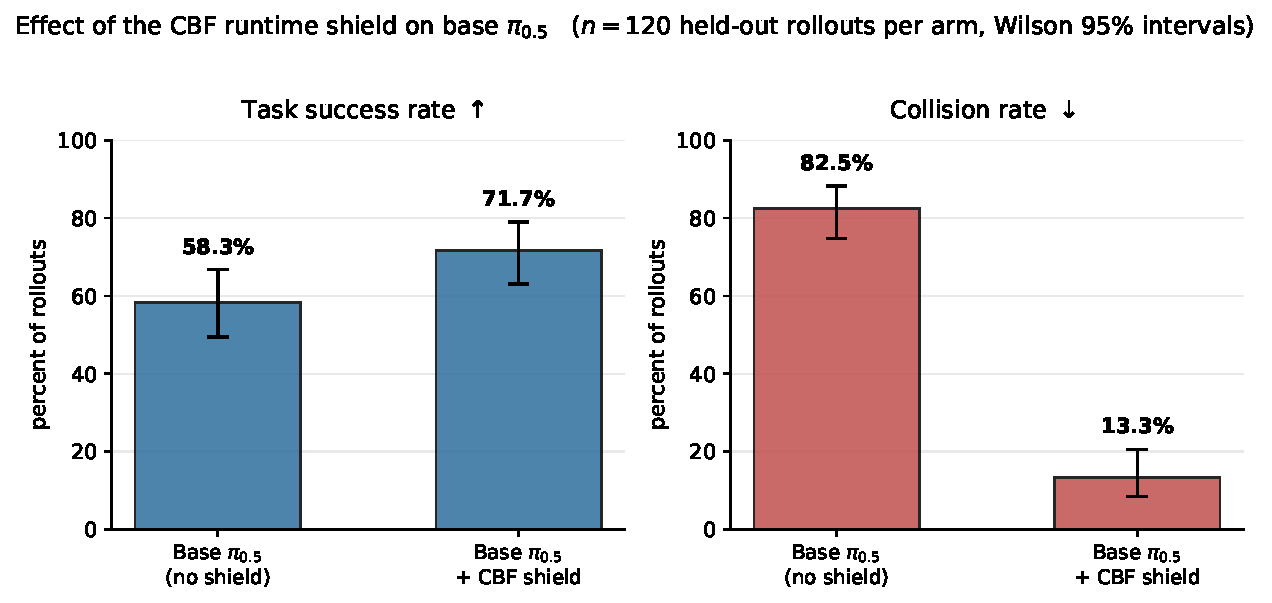
\includegraphics[width=\linewidth]{figures/fig_shield_efficacy.pdf}
  \caption{Effect of the CBF runtime shield on base $\pi_{0.5}$, pooled over all 24 scenes.
    Error bars are Wilson 95\% intervals at $n = 120$ per condition.}
  \label{fig:shield_efficacy}
\end{figure}

Unshielded, $\pi_{0.5}$ displaces the obstacle in 82.5\% of episodes. With the shield active this
falls to 13.3\%, a reduction of 69 percentage points with disjoint confidence intervals.

Success also rises, from 58.3\% to 71.7\%. This is not incidental: a collision frequently derails
the episode, knocking the target object out of reach or displacing the goal, so preventing
collisions helps the policy complete the task. This point is worth holding onto, because in
Section~\ref{sec:internalise} the same shield applied to an already-avoidant policy has the
opposite effect on success, and the two observations are only consistent once the mechanism is
stated.

\paragraph{Caveat on privileged information.}
The barrier is constructed from ground-truth obstacle geometry taken directly from the simulator,
not from perception. A deployed system would have to estimate that geometry from sensors and would
inherit the resulting error. The numbers here should therefore be read as an upper bound on what
this class of shield achieves, with the perception gap removed by construction.

\paragraph{External validation.}
The evaluation pipeline can be checked against the figures reported for $\pi_{0.5}$ by the work
that introduced \texttt{SafeLIBERO}. Table~\ref{tab:external_validation} places the two side by
side. The unshielded rows agree to within a fraction of a point on both metrics, which supports the
view that this pipeline recovers the published baseline rather than producing an artefact of the
present implementation --- a check worth making explicitly, since every subsequent result in this
chapter is measured relative to that baseline.

The shielded rows diverge, and the divergence is worth stating rather than smoothing: the shield
used here is roughly fifteen points safer and three points less successful. Two deliberate
differences in the constraint account for it. The published formulation, by its authors' own
statement, ``solely constrains the end-effector'', and its limitations section notes that
unconstrained kinematic links may consequently collide; the barrier used here additionally
constrains links three through seven and the hand body (Section~\ref{sec:barrier}), and
Section~\ref{sec:scope} shows that arm links are exactly where residual collisions concentrate.
Separately, this barrier reads ground-truth geometry from the simulator, whereas the published
layer grounds its constraints through vision-language perception and fused depth, and attributes
its own residual collisions primarily to that upstream pipeline rather than to the controller.
Both differences favour the shield used here, so these figures are an upper bound for this class of
filter rather than a like-for-like improvement over that method.

% Table 4.1 — External validation against the benchmark's originating work (AEGIS/VLSA).
% Requires: \usepackage{booktabs}  \usepackage{threeparttable}
%
% NUMBERS AND THEIR PROVENANCE:
%   This work      — figures/results_shielded_distillation.md, eval 2026-08-07, n = 120 held-out.
%   AEGIS          — their Table I, averaged over the three suites used here (spatial, goal,
%                    object). Their own averages additionally include a Long suite, so these are
%                    recomputed three-suite figures, NOT their printed averages. Verified against
%                    the PDF 2026-08-18; see papers/FINDINGS.md.
%   Do NOT cite 87.5% for their shielded CAR. That figure came from a docstring in their released
%   code, not the paper, and is wrong. The paper's three-suite figure is 71.9%.

\begin{table}[htbp]
\centering
\begin{threeparttable}
\caption[External validation against the published baseline]{%
  External validation. The unshielded baseline measured here reproduces the published
  $\pi_{0.5}$ figures to within a fraction of a point on both metrics, indicating that the
  evaluation pipeline recovers the published result rather than an artefact of this
  implementation. The shielded rows are \emph{not} like-for-like and are discussed below.}
\label{tab:external_validation}
\begin{tabular}{llcc}
\toprule
\textbf{Condition} & \textbf{Source} & \textbf{CAR} & \textbf{TSR} \\
\midrule
\multirow{2}{*}{Base $\pi_{0.5}$, no shield}
  & Published\tnote{a}      & 17.3\%          & 58.9\%          \\
  & This work\tnote{b}      & \textbf{17.5\%} & \textbf{58.3\%} \\
\addlinespace[2pt]
\multicolumn{2}{l}{\emph{difference}} & $0.2$ pp & $0.6$ pp \\
\midrule
\multirow{2}{*}{With runtime CBF shield}
  & Published\tnote{a}      & 71.9\%          & 74.6\%          \\
  & This work\tnote{b}      & 86.7\%          & 71.7\%          \\
\addlinespace[2pt]
\multicolumn{2}{l}{\emph{difference}\tnote{c}} & $+14.8$ pp & $-2.9$ pp \\
\bottomrule
\end{tabular}
\begin{tablenotes}[flushleft]\footnotesize
\item[a] Averaged over the three suites used in this work (spatial, goal, object) from the
  originating work's reported per-suite results in the full action space. Their printed averages
  additionally include a Long suite and are therefore not directly quoted here.
\item[b] $n = 120$ held-out rollouts, pooled over 24 scenes. CAR is the complement of the collision
  rate defined in Section~\ref{sec:metrics}; note that the originating work defines collision
  avoidance as the proportion of strictly collision-free episodes without stating a numeric
  tolerance, so the 1\,mm threshold used here is this work's operationalisation of that definition.
\item[c] The shielded rows are not a like-for-like comparison and the gap is expected. Two
  differences in the constraint account for it, both deliberate: the published formulation
  constrains only the end-effector, by its authors' own statement, whereas the barrier used here
  additionally constrains links three to seven and the hand (Section~\ref{sec:barrier}); and this
  barrier reads ground-truth geometry from the simulator, whereas theirs is grounded through
  vision-language perception and fused depth, to which they attribute their own residual
  collisions. Both differences favour the shield used here, so these figures are an upper bound
  for this class of filter rather than an improvement over that method.
\end{tablenotes}
\end{threeparttable}
\end{table}

